\documentclass[12pt]{article}

\usepackage{sbc-template}

\usepackage{graphicx,url}

\usepackage[brazil]{babel}
\usepackage[utf8]{inputenc}


\sloppy

\title{Trabalho final de Classificação e Pesquisa de Dados}

\author{Arthur Zachow\inst{1} e Felipe de Almeida Graeff\inst{1}}


\address{Instituto de Informática -- Universidade Federal do Rio Grande do Sul
  (UFRGS)\\
  Caixa Postal 15.064 -- 91.501-970 -- Porto Alegre -- RS -- Brazil
  \email{\{azcoelho, fagraeff\}@inf.ufrgs.br}
}

\begin{document}

\maketitle

\section{Implementação}
O trabalho foi desenvolvido na linguagem C++, padrão C++11. O código fonte pode ser visto em 
\url{https://github.com/Fxlipe115/CPD_Final}. Para o armazenamento e manipulação dos dados foi 
implementada uma tabela hash e duas classes auxiliares para a representação dos comentários e das 
palavras.

Além das funcionalidades básicas pedidas, foram implementadas as seguintes funcionalidades adicionais:

\begin{itemize}
\item Teste a partir de um arquivo de comentários.

  O arquivo de entrada deve estar no seguinte formato:
  \begin{table}[ht]
  \centering
  \begin{tabular}{|c|}
  \hline
  Comentário 1\\[0.5ex]
  Comentário 2\\[0.5ex]
  Comentário 3\\[0.5ex]
  \vdots\\[0.5ex]
  \hline
  \end{tabular}
  \end{table}

\item Melhorar a classificação dos comentários.
   
\item Buscar comentários associados a palavras.

\begin{figure}[ht]
\centering
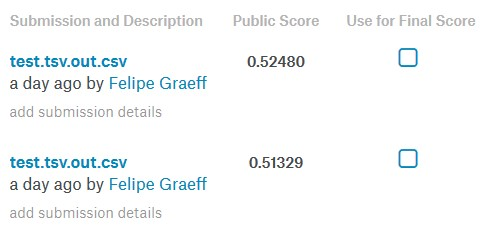
\includegraphics[width=.5\textwidth]{kaggle.jpg}
\caption{Notas dadas pelo Kaggle para a avaliação a partir de um arquivo utilizando o arquivo de 
  treinamento do Moodle (embaixo) e o arquivo train.tsv do Kaggle (em cima).}
\label{fig:kaggle}
\end{figure}
  
  
\end{itemize}

\begin{figure}[ht]
\centering
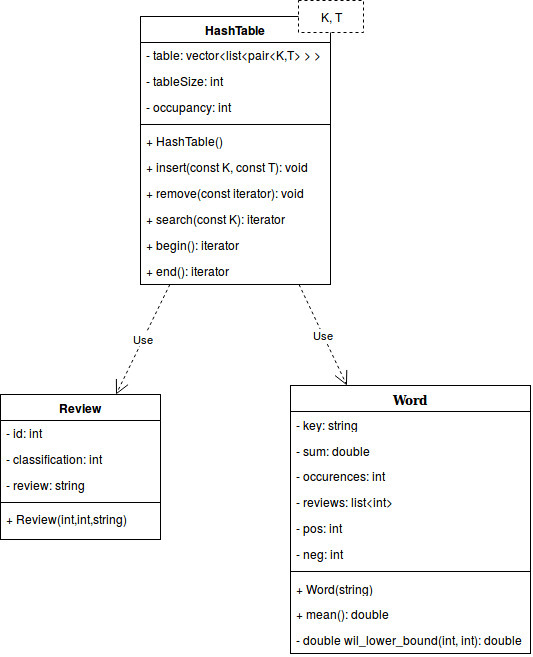
\includegraphics[width=.5\textwidth]{class_diagram.jpg}
\caption{Classes implementadas para o trabalho. Acessores e métodos auxiliares julgados irrelevantes
  para este relatório foram omitidos no diagrama.}
\label{fig:class_diagram}
\end{figure}

\subsection{Classe HashTable}

A interface da hash table implementada foi baseada na da classe std::unordered\_map da biblioteca padrão 
do C++. Isso pode ser observado no uso de parâmetros template para o tipo das chaves e dos dados e no 
uso de iteradores para as funções de busca e remoção.

Diferentemente da classe std::unordered\_map, nossa implementação utiliza encadeamento como tratamento de 
colisões (facilmente constatado pelo tipo do atributo \emph{table} da classe).



\subsection{Classe Review}

A classe Review é um classe de dados e serve apenas para armazenar os comentários lidos do arquivo de 
treinamento, o sentimento associado e uma chave numérica única.

\subsection{Classe Word}

Pode-se considerar essa como a principal classe da aplicação, pois é ela que permite o cálculo dos 
sentimentos associadas a cada palavra e, posteriormente, aos novos comentários que forem avaliados.

A classe armazena uma palavra como chave única, a soma das avaliações de todos os comentários em que 
a palavra é encontrada, assim como o número de vezes que a palavra é encontrada nos comentários de 
treinamento e uma lista contendo as chaves numéricas referentes a cada um desses comentários. Além 
disso são armazenadas a quantidade de comentários com sentimentos positivos (maiores que 2) e negativos 
(menores que 2) em que a palavra aparece. Esses dois últimos dados são importantes para o cálculo do 
score associado a cada palavra, como será visto a seguir.

\subsubsection{Intervalo de confiança de Wilson}

Para conseguir uma melhor avaliação das palavras e dos comentários foi utilizado um método estatístico 
conhecido como intervalo de confiança de Wilson. Esse método foi escolhido pois faz uma aproximação 
mais realística do que a média aritmética pedida na descrição do trabalho para o score final de cada 
palavra.

Mais especificamente, foi utilizado o limite inferior de Wilson, dado pela fórmula a seguir:

$$ w^{-} = \frac{1}{1+\frac{1}{n}z^2}\left [ \hat{p} + \frac{1}{2n}z^2 - z \sqrt{\frac{1}{n} \hat{p}
   \left ( 1 - \hat{p} \right ) + \frac{1}{4n^2} z^2} \right ] $$
   
onde $z$ determina o nível de confiança para uma certa taxa de erro, $\hat{p}$ é dado pela divisão 
entre o número de casos dentro do intervalo que se quer avaliar (os atributos \emph{neg} e \emph{pos} 
da classe Word na aplicação específica do trabalho) e o número total de casos (o atributo 
\emph{occurences}) e $n$ é o mesmo número total de casos utilizado no cálculo de $\hat{p}$.


\section{Aplicação}

Ao iniciar a aplicação é feito o preenchimento da tabela de comentários a partir do arquivo de treinamento 
e da tabela de palavras a partir de cada comentário na tabela de comentários. Para o preenchimento da tabela 
de palavras os comentários são separados em \emph{tokens}. Para isso são removidos todos os caracteres especiais 
e algarismos de cada comentários e a string resultante é passada toda para letras minúsculas e separada em 
palavras por espaços em branco. Essas palavras então geram um objeto Word que é inserido na tabela utilizando-se 
a própria palavra como chave.

Após a carga são apresentadas algumas opções ao usuário.

\begin{figure}[ht]
\centering
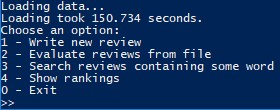
\includegraphics[width=.5\textwidth]{menu.jpg}
\caption{Menu da aplicação após carga dos dados do arquivo de treinamento.}
\label{fig:menu}
\end{figure}

\subsection{Write new review}

Essa opção avalia um comentário dado pelo usuário. Para isso é feita a mesma separação em \emph{tokens} 
que é feita para ``treinar'' o programa. Cada \emph{token} é usado para buscar o score relacionado na tabela 
de palavras. Caso a palavra digitada não exista na base da aplicação, assume-se que a palavra tem valor neutro 
(2). Após é feita a média aritmética simples dos valores retornados e o score final é informado ao usuário.

\subsection{Evaluate reviews from file}

Para essa opção cada linha do arquivo de entrada é tratada como na opção anterior e o resultado é salvo em 
um arquivo CSV de acordo com o formato determinado na plataforma Kaggle.

\subsection{Search reviews containing some word}

A palavra de entrada é transformada em um \emph{token} conforme visto anteriormente e utilizada para buscar 
o objeto Word correspondente na tabela de palavras. Então, da tabela de comentários, são retornados todos os 
comentários cuja chave esteja na lista contida no objeto Word retornado da busca anterior.

\subsection{Show rankings}

Aqui é criada uma lista com ponteiros para todos os elementos da tabela de palavras. Essa lista é então ordenada 
por um merge sort de acordo com a chave e com a ordenação requerida e os $n$ itens pedidos pelo usuário são apresentados 
a ele.

\end{document}
